\documentclass[a4paper,11pt]{article}

\usepackage{etoolbox}
\usepackage{fancyvrb}
\usepackage[T1]{fontenc}
\usepackage{graphicx}
\usepackage{import}
\usepackage{listings}
\usepackage{minted}
\usepackage{url}

\usepackage[
	% Prevent hyperlinks from getting an ugly border
    hidelinks,
    % Set proper PDF metadata
    pdftex,
    pdfauthor={Marius Schulz},
    pdftitle={Deriving Control Flow Graphs from JavaScript Programs},
    pdfsubject={How to derive the static control flow graph from a JavaScript program's abstract syntax tree},
    pdfkeywords={Control Flow Graphs, JavaScript}
]{hyperref}

\usepackage{sections/_meta/tumlogo}

% Don't display "References" when rendering the bibliography
\patchcmd{\thebibliography}{\section*{\refname}}{}{}{}

% Use appropriate font size for line numbers in listings
\renewcommand{\theFancyVerbLine}{{\small\arabic{FancyVerbLine}}}

\lstset{basicstyle=\ttfamily}
\newcommand{\code}[1]{\texttt{#1}}

\setlength{\footnotesep}{0.4cm}
\setlength{\skip\footins}{0.5cm}

\def\doctype{Bachelor's Thesis in Informatics}
\def\title{Deriving Control Flow Graphs \\ from JavaScript Programs}
\def\germantitle{Herleitung von Kontrollflussgraphen \\ aus JavaScript-Programmen}
\def\author{Marius Daniel Schulz}
\def\date{August 15, 2015}

\begin{document}

\thispagestyle{empty}

\def\bcorcor{0.15cm}
\addtolength{\hoffset}{\bcorcor}

\thispagestyle{empty}

\vspace{4cm}

\begin{center}
  \oTUM{4cm}
  
  \vspace{5mm}
  
  \huge DEPARTMENT OF INFORMATICS\\
  
  \vspace{0.5cm}
  
  \large TECHNISCHE UNIVERSIT{\"A}T M{\"U}NCHEN\\
  
  \vspace{1mm}
\end{center}

\vspace{15mm}

\begin{center}
  {\Large \doctype}

  \vspace{20mm}

  \setlength\lineskip{8pt}
  {\LARGE \bf \title}\\%[3ex]

  \vspace{15mm}

  {\LARGE \author}

  \vspace{10mm}
  
  \begin{figure}[h!]
    \centering
    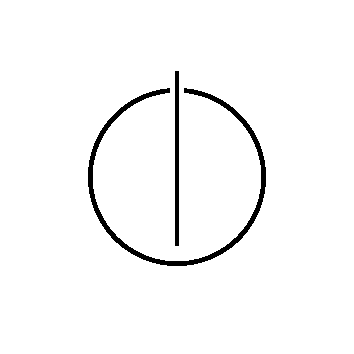
\includegraphics[width=4cm]{sections/_meta/informat.png}
  \end{figure}
\end{center}

\thispagestyle{empty}

\def\bcorcor{0.15cm}
\addtolength{\hoffset}{\bcorcor}

\thispagestyle{empty}

\vspace{4cm}

\begin{center}
  \oTUM{4cm}
  
  \vspace{5mm}
  
  \huge DEPARTMENT OF INFORMATICS\\
  
  \vspace{0.5cm}
  
  \large TECHNISCHE UNIVERSIT{\"A}T M{\"U}NCHEN\\
  
  \vspace{1mm}
\end{center}

\vspace{15mm}

\begin{center}
  {\Large \doctype}

  \vspace{20mm}

  \setlength\lineskip{8pt}
  {\LARGE \bf \title}\\%[3ex]

  \vspace{10mm}

  {\LARGE \germantitle}
\end{center}

\vfill

\renewcommand{\arraystretch}{0.7}

\begin{center}
\begin{tabular}{l@{\hskip 1cm}l}
  {\Large \bf Author:} & {\Large Marius Daniel Schulz} \\\\
  {\Large \bf Supervisor:} & {\Large Prof. Dr. Helmut Seidl} \\\\
  {\Large \bf Advisor:} & {\Large Dr. Michael Petter} \\\\
  {\Large \bf Submission date:} & {\Large 15. August 2015}
\end{tabular}
\end{center}

\thispagestyle{empty}

\vspace*{\fill}
\begin{flushright}
\noindent \textit{I confirm that this bachelor's thesis is my own work \\ and I have documented all sources and material used.\\[\baselineskip]}
M{\"u}nchen, 15. August 2015 \\[3.5\baselineskip]
\underline{\hspace{6.5cm}}
\end{flushright}


\newpage
\thispagestyle{empty}
\null

\newpage
\thispagestyle{empty}
\section*{Abstract}

 This thesis contributes to the understanding of how to derive static control flow graphs from JavaScript programs for the purpose of enabling a variety of static data flow analyses. An algorithm is presented that defines how to systematically construct a control flow graph from a program's abstract syntax tree. Furthermore, some limitations of the approach are discussed that are inherent to the dynamic nature of JavaScript. Finally, an exemplary implementation serves as a proof of concept for the applicability of the control flow graph derivation algorithm.
 

\newpage
\pagestyle{empty}
\tableofcontents

\newpage
\pagestyle{plain}
\setcounter{page}{1}

\section{Introduction}

\subsection{Motivation}
\label{sec:motivation}

When JavaScript\footnote{``JavaScript'' is a trademark of Oracle Corporation. The untrademarked name used in the language specification \cite{es5-spec} as standardized by Ecma International\textsuperscript{\textregistered} is ``ECMAScript''. Following common usage (and for ease of reference), the name ``JavaScript'' will be used hereinafter to refer to the ECMAScript language.} first appeared in 1995, it was originally envisioned to be a small scripting language for adding interactivity to web pages, which were mostly static HTML documents back then. The expected number of lines for the average script was probably in the dozens. Nowadays, JavaScript applications with several hundred thousand lines of code are being developed and maintained. The language has been brought to more and more environments and platforms over time, such as was the case with Node.js \cite{nodejs} in 2009, and it still continues to grow in usage.

As the size of programs written in JavaScript grows, so does their complexity. Large code bases are considerably harder to understand, debug, and maintain than small ones. Programmers are therefore more likely to introduce bugs into the software as the code base grows. The problem with JavaScript is that it offers little help to programmers during implementation. A dynamically typed language, JavaScript enforces neither consistent type usage nor guaranteed initialization of variables, for example. Moreover, some unfortunate language design choices\footnote{Outside of \textit{strict mode}, assigning a value to a simple identifier than cannot be resolved leads to the automatic creation of a global variable of that name. This behavior is usually unintended and does more harm than good.} may lead to unexpected and undesirable behavior at runtime.

The growing ubiquity of JavaScript and its usage in large-scale, critical applications awakens interest in techniques for automatic program verification. Static analysis tools can help developers find erroneous pieces of code by looking for patterns that, according to a given defect model, lead to commonly made mistakes. Data flow analysis, for example, inspects declarations and usages of variables in a program to track the propagation of their values. Using data flow analyses, one can try to answer the following questions:

\begin{itemize}
  \setlength\itemsep{0pt}
  \item Is there a code path that leaves a given variable uninitialized?
  \item Is the value of a given variable always within a certain range?
  \item Does a given variable always contain values of the same type?
  \item Does a given variable ever change after its initial assignment?
  \item Are there any code parts that can never be reached (dead code)?
\end{itemize}

At the heart of such data flow analyses lies the inspection of the underlying program's static control flow graph, which must therefore be derived.

\subsection{Related Work}

Recently, there has been notable related work in the area of static control flow analysis. For instance, the Flow \cite{flow} type checker developed at Facebook aims to statically find type errors in JavaScript programs. Flow analyzes plain JavaScript code, which does not have to be explicitly decorated with type annotations. The latter can optionally be included, though, to gradually improve the significance of the type checker.

Additionally, \cite{kashyap2014jsai} presents a static analysis platform for JavaScript based on JSAI, an abstract interpreter that offers user-configurable sensitivity and provably sound analysis. Due to the dynamic nature of the language, however, much work is done in the area of dynamic analyses. \cite{bichhawat2014information}, \cite{hedin2012information}, and \cite{santos2014information}, for example, focus on improving the security of JavaScript applications through dynamic information flow control.


\section{Capabilities}

This thesis outlines the derivation of intraprocedural, static control flow graphs based on a JavaScript program's abstract syntax tree. The goal is to capture the semantics of the main program or any of its functions in the respective control flow graphs, which can be used as the basis for various static data flow analyses as discussed in ``\nameref{sec:motivation}''.


\subsection{Control Flow Graph Derivation}

The derivation of a control flow graph as described in this thesis is based on a purely static analysis of the abstract syntax tree of a program. Consequently, no analysis of actual runtime behavior is performed. This limits the capabilities somewhat, since JavaScript is a highly dynamic programming language with support for language constructs that are difficult to analyze statically. Because of the highly dynamic nature of the language, the control flow graph derivation is subject to the limitations listed in section \ref{sec:limitations} (``\nameref{sec:limitations}''). Despite these difficulties, the algorithm analyzing a program's abstract syntax tree must not falsify the program semantics. It must therefore make conservative assumptions about the dynamic parts of the program in order to guarantee sound control flow analysis. Section \ref{sec:algorithm} (``\nameref{sec:algorithm}'') describes the algorithmic approach in detail. Section \ref{sec:implementation} (``\nameref{sec:implementation}'') presents an exemplary implementation that was developed as part of the work on this thesis.


\subsection{Export in Various Formats}

In addition to deriving control flow graphs, the exemplary implementation is capable of exporting its resulting data structures. A given control flow graph can be exported as a JavaScript object, which can be analyzed in the JavaScript program using the derivation library. Additionally, control flow graphs can be serialized as JSON for further processing in arbitrary tools, programming languages, and environments. Finally, the DOT export allows for serializing the structure of a control flow graph using the DOT \cite{dot-language} graph description language. Visualization tools like Graphviz \cite{graphviz} can then layout the graph and render it as an image. The different export formats are explained in sections \ref{sec:object-export} (``\nameref{sec:object-export}''), \ref{sec:json-export} (``\nameref{sec:json-export}''), and \ref{sec:dot-export} (``\nameref{sec:dot-export}''). \nameref{sec:appendix} shows examples of serialized exports in JSON and DOT format.

\section{Limitations}
\label{sec:limitations}

This section details the limitations that are an inherent part of the process of deriving an accurate control flow graph from a JavaScript program. They mainly revolve around dynamic language features, closure and scope management, and implicit errors.

\subsection{Dynamic Language Features}

A highly dynamic programming language, JavaScript supports various language constructs that are difficult or even impossible to analyze statically. Two examples are string-based access to object properties and the evaluation of strings as code. If the strings in question depend on environment variables such as time, user input, or external data, it is generally undecidable which piece of code is going to be executed.

\subsubsection{String-Based Property Access}

JavaScript offers a lightweight syntax for creating object literals. Objects consist of properties that map string keys to arbitrary values. This includes functions too, which are first-class citizens in JavaScript:

\begin{minted}[linenos,xleftmargin=0.75cm]{js}
var calculator = {
    increment: function(x) {
        return x + 1;
    },
    square: function(x) {
        return x * x;
    }
};
\end{minted}

There are two ways to access an object's properties. The first option is to use \textit{dot notation} as known from other languages with a C-like syntax:

\begin{minted}[linenos,xleftmargin=0.75cm]{js}
var two = calculator.increment(1);
\end{minted}

The other option is to use the property's string key in conjunction with \textit{square bracket notation} that looks for a property with exactly that key:

\begin{minted}[linenos,xleftmargin=0.75cm]{js}
var two = calculator["increment"](1);
\end{minted}

No matter which of the two notations was used to look up the property, the value \code{undefined} is returned if neither the object itself nor any of the objects in its \emph{prototype chain}\footnote{See section 4.2.1 of the ECMAScript Language Specification. \cite{es5-spec}} define a property with the given key. The above invocations of the \code{increment} method would have failed with a \code{TypeError} if the property lookup returned any value that was not a function.

The difficulty of statically analyzing code that accesses object properties using string keys and square bracket notation lies in the observation that it is generally undecidable which (if any) property's value is returned. In the above example, it is trivial for a static analyzer to recognize that the provided key is a string literal with a known constant value. However, the JavaScript grammar allows an arbitrary expression to be placed within the square brackets of the property access; the result of evaluating this expression is then coerced into a string and used as a property key. The following four examples show how different the results of invoking a method accessed this way can be, depending on the value of the property key:

\begin{itemize}
  \item If \code{key} contains the value \code{"increment"}, calling \code{calculator[key](5)} will return the value \code{6}. Similarly, if \code{key} is set to \code{"square"}, calling \code{calculator[key](5)} will return the value \code{25}.
  \item If \code{key} is set to \code{"hasOwnProperty"}, calling \code{calculator[key](5)} will look for and invoke the \code{hasOwnProperty} method defined on the \code{Object} prototype, which returns \code{false} because the object does not define a property with that key.
  \item If \code{key} is set to \code{"invalid property"}, calling \code{calculator[key](5)} will trigger a lookup for a method of that name. Neither the object itself nor any other object in its prototype chain defines such a property, and therefore \code{undefined} is returned. Since \code{undefined} cannot be invoked as a function, a \code{TypeError} is thrown.
\end{itemize}

This illustrates nicely how drastically the control flow behavior can vary depending on the value of the expression within the square brackets. In cases where the key is set to \code{"increment"}, \code{"square"}, or the name of any method in the prototype chain, that method will be executed. If, however, the key cannot be found, an exception will be thrown, thereby causing an abrupt completion and a jump in control flow.

\pagebreak
\subsubsection{Evaluating Strings As Code}

In addition to allowing string-based access to object properties, JavaScript provides other language mechanisms that lead to highly dynamic code execution. The most obvious such construct is the global \code{eval} function that evaluates a given string as code:

\begin{minted}[linenos,xleftmargin=0.75cm]{js}
var count = 0;
eval("count++;");
\end{minted}

After running the above code, \code{count} contains the value \code{1}. The string passed to the \code{eval} function can contain any sequence of statements or expressions, including calls to \code{eval} itself. Generally speaking, that makes it impossible for a static analyzer to understand what statements and expressions are being executed in what order. To further complicate matters, the string that is being evaluated does not have to be a string literal with a known constant value. It can be the result of any expression evaluating to a string, similar to dynamic property keys.

Another difficulty is that in some cases, it is not even possible to statically decide whether a program calls the \code{eval} function anywhere. The following code snippets illustrates how dynamic property access is used to access the \code{eval} function without explicitly mentioning its name:

\begin{minted}[linenos,xleftmargin=0.75cm]{js}
var obj = window;
var key = String.fromCharCode(101, 118, 97, 108);
var result = obj[key]("2 + 2");
\end{minted}

The global object within a browser environment, \code{window}, is assigned to the variable \code{obj}. At the same time, \code{key} is assigned the value \code{"eval"} by creating a string from the given Unicode values, which represent the four characters \textit{e}, \textit{v}, \textit{a}, and \textit{l}. Finally, the dynamic property access returns the \code{eval} function defined on the global object and evaluates the string \code{"2 + 2"}. Therefore, \code{result} contains the value \code{4}.

The following example illustrates the unpredictability of evaluating arbitrary JavaScript code using the \code{eval} function:

\begin{minted}[linenos,xleftmargin=0.75cm]{js}
var hasEvalBeenRun = false;

function runEval(string) {
    eval(string);
    hasEvalBeenRun = true;
}

runEval("var hasEvalBeenRun;");
\end{minted}

Looking at the variable declaration and the \code{runEval} function, one might assume that \code{hasEvalBeenRun} is set to \code{true} after the function has been executed (and given that running \code{eval} did not throw an exception). This does not have to be the case, though, as the example shows. By evaluating the string \code{"var hasEvalBeenRun;"} within the function, a new local variable binding is created that \emph{shadows} the outer variable of the same name. Thus, the assignment does not modify the outer variable, but the local one.

\subsubsection{Dynamically Creating Functions}

Another dynamic language construct is the \code{Function} constructor, which makes it possible to define new functions at runtime. It accepts an arbitrary number of string parameters, the last of which represents the function body. All other parameters are treated as the names of the function's formal arguments, in the order in which they are passed. \cite{mdn-function}

The following code snippet shows how a simple \code{add} function can be created by calling the \code{Function} constructor with two argument names and a function body calculating and returning the sum of the given values:

\begin{minted}[linenos,xleftmargin=0.75cm]{js}
var add = new Function("a", "b", "return a + b;");
\end{minted}

Similar to the evaluation of strings as code using the \code{eval} function, the \code{Function} constructor poses a problem for static analyzers. The string representation of the function body does not have to be a string literal, which would have a constant value. Typically, the \code{Function} constructor is used to create a function whose body is put together using dynamic string concatenation of code fragments. In general, this makes it impossible to predict statically what the body of the function will look like.

\pagebreak
\subsection{Implicitly Thrown Errors}
\label{sec:implicitly-thrown-errors}

In JavaScript, exceptions can be thrown explicitly using the \code{throw} keyword. When an exception is thrown, none of the statements following the \code{throw} statement will be executed. Instead, control will be passed to the first \code{catch} block in the call stack. If no such \code{catch} block exists, the exception will cause the program to terminate. \cite{mdn-throw}

However, the absence of \code{throw} statements within a piece of code does not guarantee that no error will be thrown within it. For instance, the following situations (and many others that are not listed below) cause the JavaScript runtime to throw an error:

\begin{itemize}
  \item A \code{ReferenceError} is thrown when trying to dereference a variable that has not previously been declared. \cite{mdn-referencerror}
  \item A \code{SyntaxError} is thrown when the JavaScript engine detects syntactically invalid code during its initial parsing phase. \cite{mdn-syntaxerror}
  \item A \code{TypeError} is thrown when a variable that does not hold a reference to a function is attempted to be called as a function. \cite{mdn-typeerror}
\end{itemize}

This list is by far not exhaustive, but it illustrates that many common operations may cause an error to be thrown implicitly. Consequently, the control flow graph for a piece of code would have to include error transitions from every single node that could possibly cause an error to either a \code{catch} handler or the error exit node of a program. That would result in many additional edges and an even more cluttered control flow graph. It is for this reason that the implementation outlined in section \ref{sec:implementation} (``\nameref{sec:implementation}'') does not include transitions for implicitly thrown errors.


\section{Algorithm}
\label{sec:algorithm}

This section illustrates the algorithmic approach used to derive a static control flow graph from a JavaScript program. It describes the graph format and how to parse statements and expressions. This section also discusses techniques for simplifying negated conditions where possible.


\subsection{Obtaining the Abstract Syntax Tree}

The algorithm for deriving static control flow graphs does not operate on the JavaScript program's raw source code, but on its abstract syntax tree. Therefore, a JavaScript parser is required to parse the program and return its abstract syntax tree, which then serves as the basis for control flow graph derivation. While the format of the abstract syntax tree can vary between parsers, the following sections assume the ESTree \cite{estree-spec} format (without loss of generality). ESTree describes a simple format that covers the entire ECMAScript 5.1 grammar, and it is implemented by popular open-source JavaScript parsers such as Acorn \cite{acorn} or Esprima \cite{esprima}. The control flow graph derivation library described in section \ref{sec:implementation} (``\nameref{sec:implementation}''), for instance, uses Esprima to obtain an abstract syntax tree in ESTree format.

\nameref{sec:appendix} shows an exemplary JavaScript program and its abstract syntax tree as generated by Esprima.


\subsection{Deriving a Control Flow Graph}

Once the abstract syntax tree of a program has been generated, it can be traversed to successively construct the control flow graph.

\subsubsection{Graph Format}

The control flow graph is a directed graph that is generally not acyclic because of cycles created by loop structures. Its nodes represent states of the program, whereas its edges represent transitions between those states. Edges can be annotated with statements or expressions that change the state of the program. Here is an example of a very simple control flow graph:

\begin{figure}[h]
  \centering
  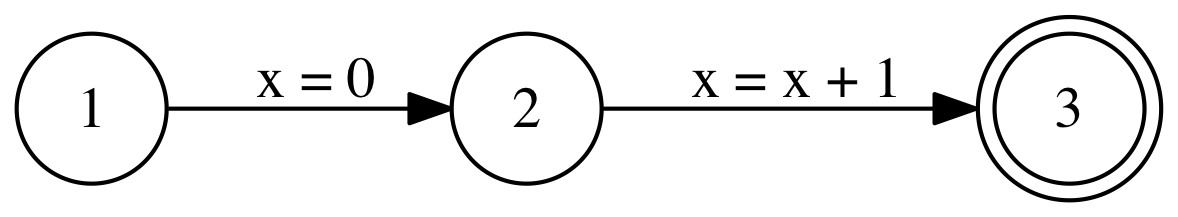
\includegraphics[width=0.7\textwidth]{sections/algorithm/images/simple-cfg}
\end{figure}

It represents the following simple JavaScript program:

\begin{minted}[linenos,xleftmargin=0.6cm]{js}
var x = 0;
x = x + 1;
\end{minted}

The abstract syntax tree in ESTree format looks like this:

\begin{minted}[linenos,baselinestretch=0.93,xleftmargin=0.75cm]{json}
{
  "type": "Program",
  "body": [
    {
      "type": "VariableDeclaration",
      "declarations": [
        {
          "type": "VariableDeclarator",
          "id": {
            "type": "Identifier",
            "name": "x"
          },
          "init": {
            "type": "Literal",
            "value": 0
          }
        }
      ],
      "kind": "var"
    },
    {
      "type": "ExpressionStatement",
      "expression": {
        "type": "AssignmentExpression",
        "operator": "=",
        "left": {
          "type": "Identifier",
          "name": "x"
        },
        "right": {
          "type": "BinaryExpression",
          "operator": "+",
          "left": {
            "type": "Identifier",
            "name": "x"
          },
          "right": {
            "type": "Literal",
            "value": 1
          }
        }
      }
    }
  ]
}
\end{minted}

\subsubsection{Parsing Statements and Expressions}

Every JavaScript program's abstract syntax tree in ESTree format has a root node of type \code{Program} with a \code{body} property that contains an array of all the main program's statements. The simple JavaScript program at the end of the previous section consists of two statements: a variable declaration and an expression statement. \code{x = x + 1} is an assignment expression and therefore not a statement on its own, but since it appears in statement position, the expression is treated as a statement of type \code{ExpressionStatement}.

The process of traversing the abstract syntax tree and deriving a control flow graph from the statements and expressions encountered can be nicely broken up into many functions, each of which knows how to parse a specific node type. One such function can call another to parse the various components of the node it knows how to parse, thereby creating a hierarchy of nested function calls. For example, the aforementioned program could be parsed by a function call hierarchy similar to the following pseudocode:

\begin{Verbatim}[xleftmargin=0.5cm]
- parseProgram()
    - parseStatements()
        - parseStatement()
            - parseVariableDeclaration()
                - parseVariableDeclarators()
                    - parseVariableDeclarator()
                        - parseInit()
                            - parseExpression()
                                - parseLiteral()
                        - parseIdentifier()
        - parseStatement()
            - parseExpressionStatement()
                - parseExpression()
                    - parseAssignmentExpression()
                        - parseRightHandSide()
                            - parseBinaryExpression()
                                - parseLeftHandSide()
                                    - parseIdentifier()
                                - parseRightHandSide()
                                    - parseLiteral()
                                - parseOperator()
                        - parseLeftHandSide()
                            - parseIdentifier()
                        - parseOperator()
\end{Verbatim}

In most cases, every expression statement adds to the control flow graph a new node with an incoming edge that is annotated with the expression. An exception to that rule, however, are expression statements that wrap expressions of type \code{SequenceExpression}.\footnote{A sequence expression as specified by ESTree \cite{estree-spec} consists of two or more expressions, separated by the comma operator, and evaluates to the value of its last expression.} Rather than adding a single node, an individual node is added for each expression in the sequence, which slightly reduces the complexity of those edge annotations in the control flow graph.

\subsubsection{Composing Structural Patterns}
\label{sec:composing-structural-patterns}

A control flow graph is created by composing various primitive patterns for statements and expressions. The following figures show a couple of examples for common control structures like conditions and loops:

\begin{figure}[h]
  \centering
  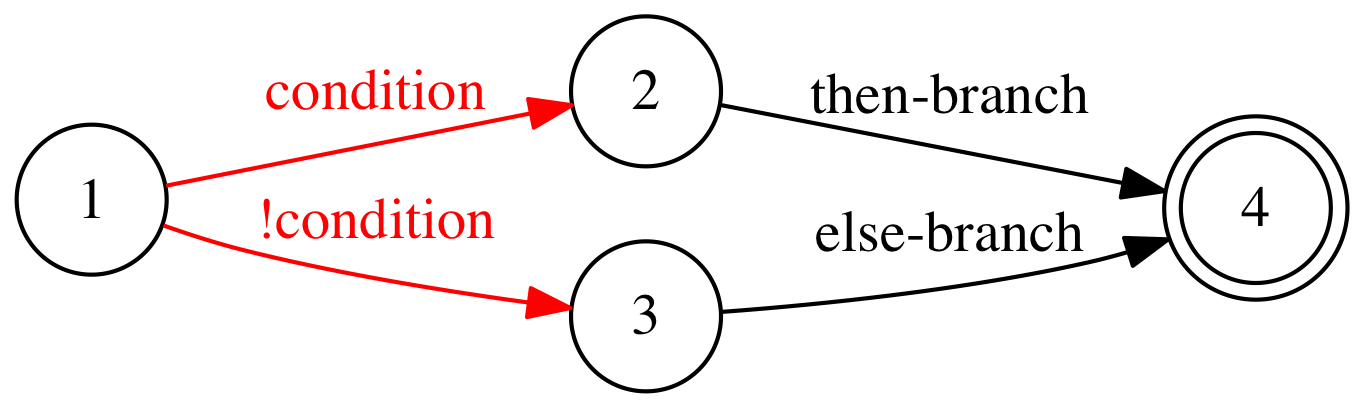
\includegraphics[width=0.7\textwidth]{sections/algorithm/images/if-else}
  \caption{An \code{if}-statement with an \code{else}-block}
  \label{fig:if-else-structural-pattern}
\end{figure}

\begin{figure}[h]
\noindent\begin{minipage}[t]{0.50\textwidth}
  \centering
  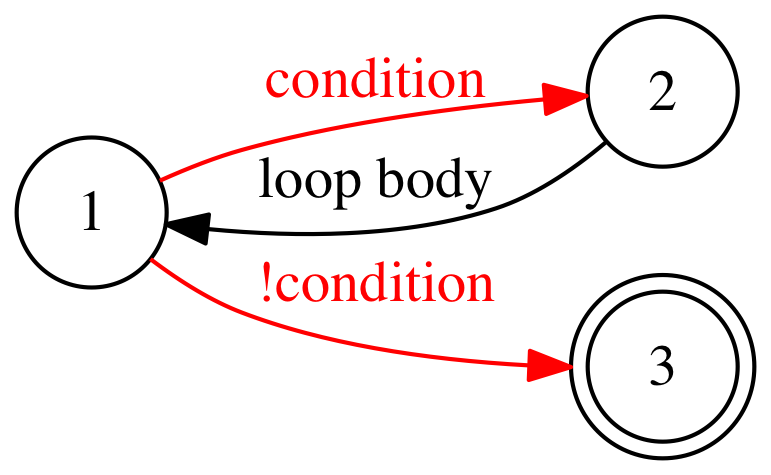
\includegraphics[width=0.8\textwidth]{sections/algorithm/images/while}
  \caption{A \code{while}-loop}
\end{minipage}
\begin{minipage}[t]{0.50\textwidth}
  \centering
  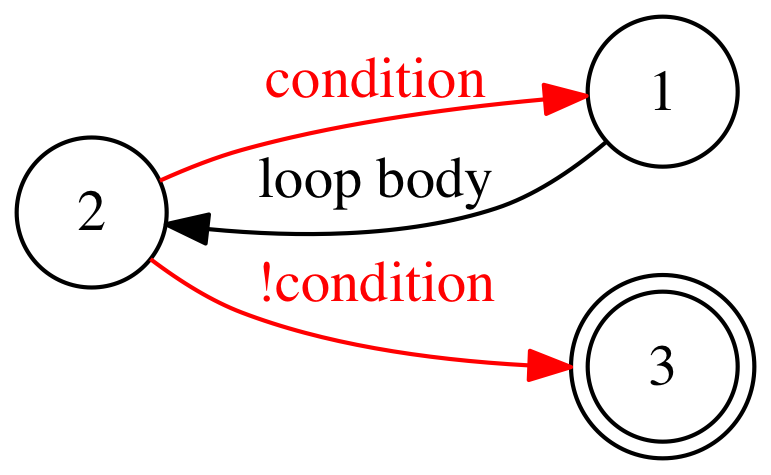
\includegraphics[width=0.8\textwidth]{sections/algorithm/images/do-while}
  \caption{A \code{do-while}-loop}
\end{minipage}
\end{figure}

\begin{figure}[h]
  \centering
  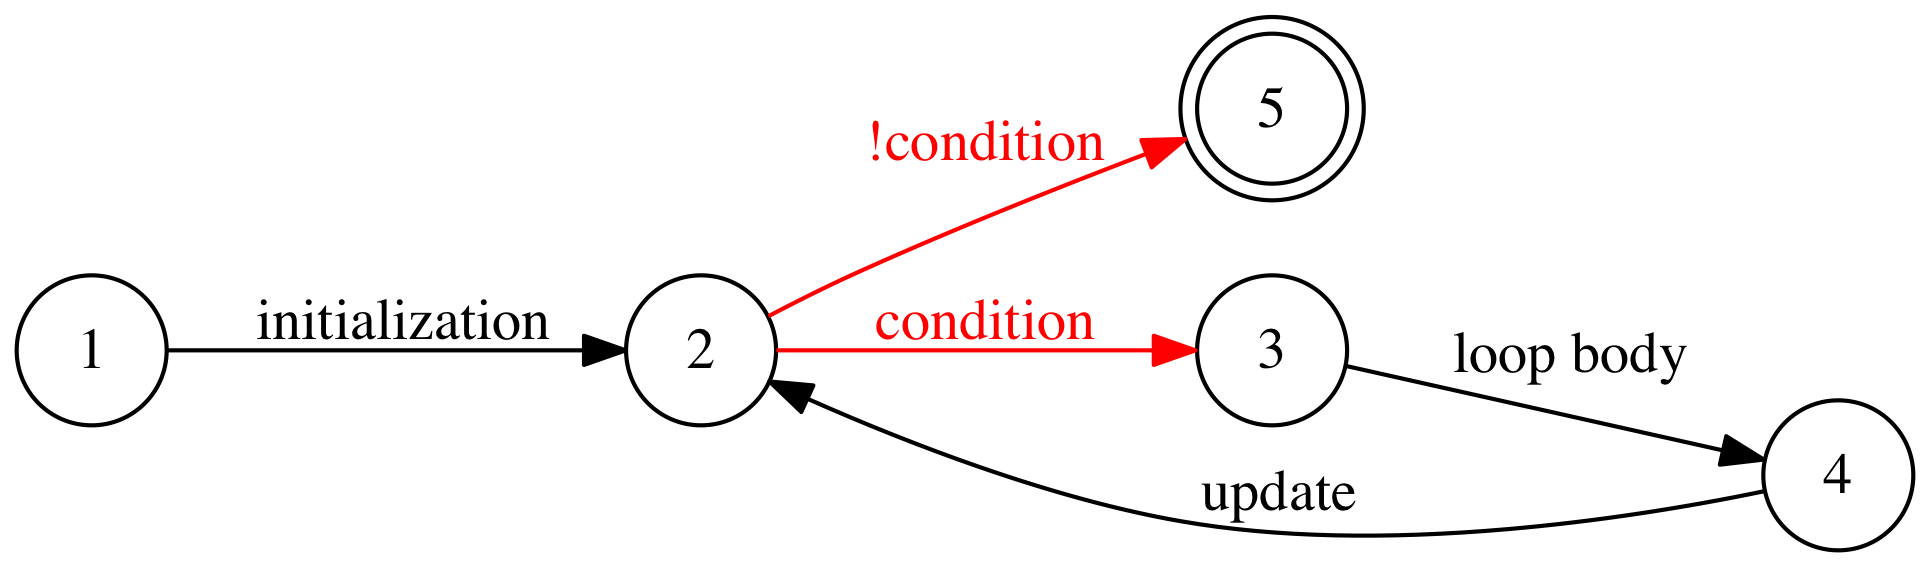
\includegraphics[width=\textwidth]{sections/algorithm/images/for}
  \caption{A \code{for}-loop}
\end{figure}

Each pattern starts with node \#1 and ends with the node that has a double border. In the above figures, those final nodes only have a double border for the purposes of clarification; they are regular nodes in the control flow graph. When two consecutive patterns are combined, the final node of the first becomes the entry node of the second. The black edges that are labeled \emph{then-branch}, \emph{else-branch}, and \emph{loop body} represent the bodies of the control structures. They can consist of arbitrarily many statements, which can contain further nested structures themselves. Similarly, \emph{initialization} and \emph{update} can hold arbitrarily complex expressions. For example, a \code{for}-loop can have a sequence expression like \code{i++, j-{}-} as its update component.

The red edges represent conditional transitions. A node that is not a final node must have either exactly one unconditional outgoing edge or exactly two conditional outgoing edges. For a pair of conditional edges, the condition is evaluated only once. Depending on whether the result is truthy or falsy\footnote{JavaScript has six values that are considered falsy: \code{undefined}, \code{null}, \code{false}, \code{0} (zero), \code{NaN} ("not a number"), and \code{""} (empty string). All other values are considered truthy.}, the corresponding conditional edge is taken.

\nameref{sec:appendix} presents a larger program and its control flow graph.

\subsubsection{Simplifying Negated Conditions}

As Figure \ref{fig:if-else-structural-pattern} in section \ref{sec:composing-structural-patterns} (``\nameref{sec:composing-structural-patterns}'') shows, an \code{if}-statement with an \code{else}-block is represented by a control flow structure that has two conditional edges. One is taken when the condition is truthy (the \emph{then-branch}), the other when it is falsy (the \emph{else-branch}). The following listing illustrates this situation:

\begin{minted}[linenos,xleftmargin=0.75cm]{js}
if (x < 0) {
    // ...
} else {
    // ...
}
\end{minted}

The then-branch is taken when \code{x < 0} returns a truthy value. It might therefore seem intuitive to assume the else-branch to be taken if and only if \code{x >= 0} is truthy. However, the precise semantics are slightly different. The else-branch is taken if and only if \code{x < 0} returns a falsy value. In general, the correct negation of \code{x < 0} is not \code{x >= 0}, but \code{!(x < 0)}. The reason for this seemingly odd behavior is that JavaScript defines some special values for which no reasonable comparison can be done using relational operators. \code{NaN} and \code{undefined} are two such values for which no sound order relation is defined.

\newpage

The following relational comparisons against \code{NaN} and \code{undefined} illustrate why the condition cannot be safely inverted (without changing the semantics of the program) by swapping the operator accordingly:

\begin{minted}[linenos,xleftmargin=0.75cm]{js}
NaN <  0   // false
NaN >  0   // false
NaN <= 0   // false
NaN >= 0   // false

undefined <  0   // false
undefined >  0   // false
undefined <= 0   // false
undefined >= 0   // false
\end{minted}

This observation prevents some simplification of conditional edges in a control flow graph. To stay true to the program semantics, the conditional annotation of the edge transitioning into the else-branch must be \code{!(x < 0)} (rather than the simpler \code{x >= 0}) to account for those special values.

However, some simplification of expressions is possible. Both the equality comparison operators (\code{==} and \code{!=}) and the identity comparison operators (\code{===} and \code{!==}) can safely be negated by flipping the first character from an equal sign to an exclamation mark, and vice-versa. Also, two consecutive applications of the unary negation operator (\code{!}) cancel each other out and do not affect the truthiness of a value. Therefore, the following simplifications are safe and do not affect the semantics of the program:

\begin{minted}[linenos,xleftmargin=0.75cm]{js}
// Simplifying a negated identity comparison
!(x === 0)
x !== 0

// Simplifying a negated inequality comparison
!(x != 0)
x == 0

// Canceling out a double negative
!!(x)
x
\end{minted}

Nota bene: The above simplifications are only semantically correct w.r.t. the evaluation of the expression to a truthy or falsy value, as is the case when evaluating the condition of an \code{if}-statement. The simplifications do not necessarily result in an identical value or even a value of the same type. For instance, the unary negation operator coerces its operand into a boolean value. Therefore, \code{!!0}, which evaluates to the boolean value \code{false} (because \code{!0} evaluates to \code{true}), is not identical to \code{0}, which is a numeric value. Both are falsy values, though, and thus direct control flow correctly.


\section{Implementation}
\label{sec:implementation}

As part of this thesis, the outlined algorithm for deriving control flow graphs has been implemented. The resulting JavaScript program consists of two main parts: the \textit{Styx}\footnote{The library was named after the river Styx, which in Greek mythology is believed to form the boundary between Earth and the Underworld.} core library that implements the control flow graph derivation (discussed in section \ref{sec:styx-corelib}) and a command-line application that provides a wrapper around the core library (discussed in section \ref{sec:styx-cli}). 

\subsection{Technology Stack}

The following sections give an overview of the programming languages and build tools that were used to implement and build the Styx core library and the wrapping command-line application.

\subsubsection{Programming Languages}

When choosing the technology stack to build upon, the goal was to develop a piece of software that could run in any modern JavaScript environment, including both Node.js and all major browsers' JavaScript engines. Taking that into account, an adequate language version to target is ECMAScript 5, which was standardized \cite{es5-spec} in 2009. Now in 2015, it is widely supported in various environments and therefore a suitable language target.

However, the Styx core library is not written in JavaScript directly, but in TypeScript \cite{typescript}, a superset of JavaScript that adds optional static typing to the language. After the TypeScript compiler has found a given program to be type-correct, it emits an equivalent JavaScript program with all type annotations removed. Therefore, the type information is a purely compile-time artifact without any runtime manifestation. The decision in favor of TypeScript was made to take advantage of the following benefits:

\begin{enumerate}
  \item Static typing helps detect a certain class of errors at compile-time by checking that a program is written in a type-correct manner. This is especially helpful in a dynamic language like JavaScript, which allows any function to be called with an arbitrary number of arguments.
  \item TypeScript supports the new ECMAScript 2015 language version that was standardized \cite{es2015-spec} in June of 2015. It adds a plethora of features to JavaScript, such as a native module system, lexical scoping, arrow functions, destructuring, and more. The TypeScript transpiler is capable of down-leveling most new language features such that engines implementing ECMAScript 5 can understand them. This allows for using next-generation JavaScript without sacrificing compatibility.
\end{enumerate}

\subsubsection{Build Tools}
\label{sec:build-tools}

To build Styx from source, both the TypeScript compiler and the Browserify module bundler \cite{browserify} must be run as discussed in the following paragraphs.

\paragraph{TypeScript Compiler.}
Since the entire code base for the Styx core library is written in TypeScript, it needs to be transpiled to plain JavaScript before it can be executed by a JavaScript engine. The official TypeScript compiler, \textit{tsc}, is used to accomplish that. It ships as part of the npm \cite{npm} package \texttt{typescript}, which can be installed by running the following command:

\begin{minted}[xleftmargin=0.75cm]{text}
$ npm install --global typescript
\end{minted}

The \texttt{src} directory of the code base contains a special \texttt{tsconfig.json} file that specifies configuration settings for the TypeScript compiler, such as the list of files to include and which compiler flags to set. During development, the compiler is run in \textit{watch} mode via the \texttt{-w} flag: every time a \texttt{.ts} file changes on disk, the TypeScript compiler will type-check and transpile it. The generated JavaScript code is then written to a \texttt{.js} file located within the destination folder that is specified in \texttt{tsconfig.json}.

\paragraph{Modules.}
To structure the code base, the Styx core library is broken up into native JavaScript modules that were introduced as part of ECMAScript 2015. As of version 1.5, the TypeScript compiler understands this syntax and is able to transpile the modules into a different format. Styx targets CommonJS modules \cite{commonjs-modules}, which is specified within \texttt{tsconfig.json} by setting the \code{module} property to \code{"commonjs"}. Following the CommonJS format, the rewritten modules declare their imports via \code{require} and their exported values via \code{exports}. Once all modules have been transpiled this way, the Styx core library is now ready to be loaded from within a Node.js application or any other JavaScript environment that supports CommonJS modules.

\paragraph{Browserify.}
While a Node.js application is able to resolve CommonJS dependencies that are imported via the \code{require} function, browsers cannot do that natively. One option to work around this issue is to use a module loader, which dynamically resolves CommonJS dependencies. The disadvantage of such module loaders is that they have to make additional HTTP requests to resolve the declared dependencies. Depending on the nesting level of \code{require} calls and the performance goals of an application, dynamically fetching CommonJS modules might not be a viable option. This is why the build process of the Styx core library includes feeding the transpiled CommonJS modules to Browserify \cite{browserify}, a popular module bundler. Starting at a given entry file, Browserify will recursively analyze all the \code{require} calls and bundle all dependencies found. The result is a single JavaScript file that can easily be requested by a browser.

\subsection{Core Library}
\label{sec:styx-corelib}

The key part of the implementation is the Styx core library. It implements the outlined algorithm for deriving the control flow graph from a program or function's abstract syntax tree. Styx itself does not have any dependencies. However, it requires that the abstract syntax tree it is handed follow the  ESTree \cite{estree-spec} specification. The two JavaScript parsers Acorn \cite{acorn} and Esprima \cite{esprima}, for instance, return an abstract syntax tree in ESTree format that can directly be passed along to the Styx parser.

\subsubsection{Public Interface}

Styx exposes a public interface that offers a \code{parse} method and several other methods for exporting a given control flow graph in various formats.

\paragraph{parse.} The \code{parse} method accepts as its parameters an abstract syntax tree and a parser configuration. Using these two inputs, it derives a control flow graph for each of the program's functions and also for the main program itself. It then returns all control flow graphs within a wrapping data structure that is called a \textit{flow program}. The first parameter of the \code{parse} method, \code{ast}, represents the abstract syntax tree to be parsed. It is a required parameter that must comply with the \texttt{Program} format as specified by ESTree. Additionally, the optional second parameter \code{options} can be provided to configure which optimization passes to apply to each control flow graph of the flow program.

\paragraph{exportAsObject.} The \code{exportAsObject} method accepts a single parameter named \code{flowProgram} that has been returned from the \code{parse} method. It exports the given program and all its functions as a JavaScript object structure that holds all nodes and edges in flat arrays rather than nested object structures, thus allowing for simpler serialization and deserialization. The \code{exportAsObject} method is discussed in detail in section \ref{sec:object-export}.

\paragraph{exportAsJson.} Similar to the \code{exportAsObject} method, \code{exportAsJson} takes a flow program and converts it to a JavaScript object with a different structure. However, \code{exportAsJson} does not return the new object itself, but a string containing its JSON representation. An optional settings parameter allows for customization of the JSON indentation. \code{exportAsJson} is explained in section \ref{sec:json-export}.

\paragraph{exportAsDot.} Lastly, the \code{exportAsDot} method  exports a single control flow graph in DOT format. The resulting graph description can be passed along to a visualization tool to render an image of the given control flow graph. \code{exportAsDot} is detailed in section \ref{sec:dot-export}.

\subsubsection{Object Export}
\label{sec:object-export}

When a flow program is exported as a JavaScript object, the returned value adheres to the following \textit{FlowProgram} schema:

\noindent
\begin{minipage}[t]{0.56\textwidth}
\begin{listing}[H]
\begin{minted}[xleftmargin=0.4cm]{ts}
interface FlowProgram {
    program:   MainProgram;
    functions: FlowFunction[];
}

interface MainProgram {
    flowGraph: FlowGraph;
}

interface FlowEdge {
    from:  number;
    to:    number;
    type:  string;
    label: string;
    data:  Object;
}
\end{minted}
\end{listing}
\end{minipage}\hfill
\begin{minipage}[t]{0.44\textwidth}
\begin{listing}[H]
\begin{minted}{ts}
interface FlowFunction {
    id:        number;
    name:      string;
    flowGraph: FlowGraph;
}

interface FlowGraph {
    nodes: FlowNode[];
    edges: FlowEdge[];
}

interface FlowNode {
    id:   number;
    type: string;
}
\end{minted}
\end{listing}
\end{minipage}

\paragraph{FlowProgram.}
A flow program that has been exported as a JavaScript object follows the \textit{FlowProgram} schema, which defines the two properties \code{program} and \code{functions}. The \code{program} property holds a single descriptor object for the main program. Similarly, the \code{functions} property holds an array of function descriptors, each of which stores both an \code{id} and a \code{name} property to uniquely identify the function. Both \textit{MainProgram} and \textit{FlowFunction} descriptors define a \code{flowGraph} property containing the associated control flow graph.

\paragraph{FlowGraph.}
The \textit{FlowGraph} schema defines the two properties \code{nodes} and \code{edges} that are both flat arrays. Representing a control flow graph this way has the advantage that every node and every edge only appears once in the serialized export. If, however, a node were to define an \code{outgoingEdges} property, every edge of that array would have to be part of another node's \code{incomingEdges} property as well. In that case, all edges would have been serialized twice, thus complicating the deserialization process.

\paragraph{FlowNode.}
Within the \code{nodes} array, every element follows the \textit{FlowNode} schema and therefore has a numeric \code{id} property. In addition to that, the \code{type} property is set to one of the following string values:

\begin{enumerate}
  \item \code{"Entry"} for the single entry node of a control flow graph,
  \item \code{"SuccessExit"} for its single success exit node,
  \item \code{"ErrorExit"} for its single error exit node, or
  \item \code{"Normal"} for all other nodes.
\end{enumerate} 

\paragraph{FlowEdge.}
Finally, the \code{edges} array contains all edges of the control flow graph. An edge's \code{from} and \code{to} properties describe which source and target node it connects. Similar to a node, an edge also has a \code{type} property that has one of the following string values:

\begin{enumerate}
  \item \code{"AbruptCompletion"} for an edge representing a jump in control flow caused by an abrupt completion (\code{break}, \code{continue}, \code{return}, or \code{throw}),
  \item \code{"Conditional"} for an edge that is part of a pair of edges representing the truthy and falsy paths of a condition,
  \item \code{"Epsilon"} for an edge that has neither a label nor attached data and exists purely for connecting nodes in the control flow graph, or
  \item \code{"Normal"} for all other edges.
\end{enumerate} 

The \code{label} property contains a string representation of the statement or expression for which the edge has been created. Additionally, the \code{data} property holds the part of the abstract syntax tree that Esprima parsed for the given statement or expression. That includes the precise type of the syntax tree node and all of its properties. The \code{data} property is useful when a deeper understanding of the current part of the control flow graph is required than can be obtained from the edge's string representation alone.

\subsubsection{JSON Export}
\label{sec:json-export}

The JSON export is a thin wrapper around the Object export described in the previous section. Instead of returning the raw JavaScript object itself, the \code{exportAsJson} method serializes it as JSON and returns the resulting string. \code{exportAsJson} accepts an optional second parameter that can specify a \code{pretty} property. The resulting JSON string will be indented for better readability if \code{pretty} has a truthy value; otherwise, it will be minified.\footnote{Note that the JSON string is only indented and formatted to help a human reader understand the object structure. Outside of string literals, whitespace is insignificant and is generally ignored by JSON parsers.}

\nameref{sec:appendix} lists an example of a flow programs exported as JSON.
\subsubsection{DOT Export}
\label{sec:dot-export}

Flow programs can be exported in DOT \cite{dot-language} format as well. DOT is a graph description language that can be consumed by visualization tools such as Graphviz \cite{graphviz} to render various sorts of graphs. In the case of Styx, the DOT export is a directed and generally not acyclic graph. It describes a finite state machine representing the control flow in a program or function.

In contrast to the JSON export, the DOT export does not include the entire flow program, but only a single control flow graph. Since Styx works on an \textit{intra}procedural rather than an \textit{inter}procedural level, the control flow graphs of the program and its functions are parsed separately from each other and can therefore be visualized independently.

\nameref{sec:appendix} shows an example of a control flow graph exported as DOT and its respective Graphviz rendering.

\subsubsection{Installation via npm}

In order to make the Styx library easily accessible to JavaScript developers, it has been published as a package to the npm Registry \cite{npm}, a public collection of open-source JavaScript packages. On a machine with npm set up, the library can be installed by running the following command:

\begin{minted}[xleftmargin=0.75cm]{text}
$ npm install --save styx
\end{minted}

Once the \texttt{styx} package has been installed, the library can be loaded through \code{require} calls like any npm package. A very simple example program (that also requires the \texttt{esprima} package to be installed) can look like this:

\begin{minted}[linenos,xleftmargin=0.75cm]{js}
// Import Esprima and Styx
var esprima = require("esprima");
var styx = require("styx");

// Create a string with demo code
var code = "console.log('Hello World!');";

// Generate the abstract syntax tree
var ast = esprima.parse(code);

// Derive the control flow graph
var flowProgram = styx.parse(ast);

// Export the control flow graph as JSON
var jsonExport = styx.exportAsJson(flowProgram);
console.log(jsonExport);
\end{minted}

\subsubsection{Building from Source}

The source code for Styx is published under the permissive MIT License \cite{mit-license} and is publicly available on GitHub \cite{styx-github}. To build Styx from source, the Git repository needs to be cloned on a local development machine. By running the following commands, the repository is going to be cloned into the \texttt{styx} folder, which is then made the current working directory:

\begin{minted}[xleftmargin=0.75cm]{text}
$ git clone https://github.com/mariusschulz/styx.git
$ cd styx
\end{minted}

Now that the repository has been set up, the npm dependencies declared in the special \texttt{package.json} file need to be restored. They can be installed via npm by running the \texttt{install} command without any arguments:

\begin{minted}[xleftmargin=0.75cm]{text}
$ npm install
\end{minted}

As described in the ``\nameref{sec:build-tools}'' section, the TypeScript code must be transpiled into plain JavaScript. That is most easily done by calling the TypeScript compiler with \texttt{-p} argument pointing to the directory containing the \texttt{tsconfig.json} configuration file (assuming that the current working directory is the root of the Git repository):

\begin{minted}[xleftmargin=0.75cm]{text}
$ tsc -p src
\end{minted}

To simplify the process of bundling modules using Browserify as much as possible, the Gulp \cite{gulp} build system has been set up. It defines a \code{browserify} task in its \texttt{gulpfile.js} configuration file that is found in the repository root. Additionally, the \texttt{package.json} file defines an npm script called \code{browserify} so that the module bundling can be triggered by running the following command:

\begin{minted}[xleftmargin=0.75cm]{text}
$ npm run browserify
\end{minted}

During development, it is handy to have both the TypeScript compiler and Browserify listen for file changes. When a \texttt{.ts} file is saved within the \texttt{src} folder, the TypeScript compiler will transpile it immediately and save the corresponding \texttt{.js} file within the destination directory. That, in turn, will be picked up by the Browserify listener, which will trigger the module bundling again.

To run the TypeScript compiler in watch mode, call it with the \texttt{-w} flag:

\begin{minted}[xleftmargin=0.75cm]{text}
$ tsc -p src -w
\end{minted}

The browserify listener can be started by running another npm script:

\begin{minted}[xleftmargin=0.75cm]{text}
$ npm run browserify-watch
\end{minted}


\subsection{Command-Line Interface}
\label{sec:styx-cli}

The \emph{Styx CLI} project provides a simple command-line interface that exposes the functionality of the Styx core library. It imports the Esprima \cite{esprima} parser and is therefore capable of loading a JavaScript file, generating its abstract syntax tree, and deriving a control flow graph from it.

\subsubsection{Installation via npm}

Similar to the Styx core library, the Styx command-line interface is available via npm as well. It can be installed by running the following command:

\begin{minted}[xleftmargin=0.75cm]{text}
$ npm install --global styx-cli
\end{minted}

As part of the global installation, the Styx CLI has been added to the system's PATH environment variable. It can then be accessed by calling \texttt{styx} within a terminal. The available arguments are listed in detail in section \ref{sec:styx-cli-args} (``\nameref{sec:styx-cli-args}'').

\subsubsection{Building from Source}

The source code for the Styx CLI project is available on GitHub \cite{styx-cli-github} under the MIT License, just like the core library. The process of building it from source is similar as well:

\begin{minted}[xleftmargin=0.75cm]{text}
$ git clone https://github.com/mariusschulz/styx-cli.git
$ cd styx-cli
$ npm install
\end{minted}

Unlike the core library, the Styx command-line interface is not written in TypeScript. It does, however, use ECMAScript 2015 language features that need to be transpiled to ECMAScript 5 in order to be widely supported by current Node.js installations. The Babel \cite{babel} transpiler, which is installed as part of the \texttt{gulp-babel} npm package, is used to do that. It is invoked by the Gulp build system when executing the \code{babel} task defined in the \texttt{gulpfile.js} configuration file. The Gulp \code{babel} task can be triggered by running this npm script:

\begin{minted}[xleftmargin=0.75cm]{text}
$ npm run babel
\end{minted}

Another npm script has been defined for setting up a file watcher that re-triggers the Babel transpilation process whenever a \texttt{.js} file changes:

\begin{minted}[xleftmargin=0.75cm]{text}
$ npm run babel-watch
\end{minted}

After the transpilation is done, the \texttt{built} directory contains the source files making up the Styx command-line interface. All JavaScript files have been down-leveled from ECMAScript 2015 to ECMAScript 5, ready to be executed by any current Node.js version.

\subsubsection{Command-Line Arguments}
\label{sec:styx-cli-args}

Using the Styx command-line interface installed via npm, a JavaScript file can be analyzed by running the following command:

\begin{minted}[xleftmargin=0.75cm]{text}
$ styx input.js
\end{minted}

This simple usage of the \texttt{styx} executable provides a single argument, the JavaScript file to analyze, which is the only argument that is required. The following command-line arguments are accepted:

\begin{itemize}
  \item The \texttt{-{}-format} argument (or its \texttt{-f} alias) determines the target output format. If specified, this argument must be either \texttt{json} or \texttt{dot}. If not specified, the export defaults to the JSON format.
  \item The \texttt{-{}-graph} argument (or its \texttt{-g} alias) specifies the id of the function whose control flow graph should be exported. This argument only applies when \texttt{-{}-format} is set to \texttt{dot}. If not present or set to a falsy value, the main program's control flow graph will be exported.
  \item The \texttt{-{}-minify-json} (or its \texttt{-m} alias) argument can be provided to export minified (rather than indented) JSON to minimize the size of the output. This argument only applies when \texttt{-{}-format} is set to \texttt{json}.
  \item The \texttt{-{}-output} argument (or its \texttt{-o} alias) can be used to specify a path to a file to which the output should be redirected. If not present, the serialized export will be written to standard output.
  \item The \texttt{-{}-help} argument displays a help screen that lists instructions for command-line usage and all available arguments. If the \texttt{-{}-help} argument is present, no export will happen, no matter what other arguments are specified; instead, only the help screen will be shown.
\end{itemize}

As an alternative to the \texttt{-{}-output} argument, the Unix output redirection operator (\texttt{\textgreater}) can be used to write the serialized export to a file. The following two commands are therefore semantically equivalent:

\begin{minted}[xleftmargin=0.75cm]{text}
$ styx input.js --output output.json
$ styx input.js > output.json
\end{minted}

Finally, the following command exports the control flow graph of the function with the id 42 in DOT format:

\begin{minted}[xleftmargin=0.75cm]{text}
$ styx input.js --format dot --graph 42 > output.gv
\end{minted}



\section{Future Work}

The exemplary implementation that was done as part of this thesis is mainly a proof of concept. It demonstrates the capabilities of the outlined approach for statically analyzing JavaScript programs to derive control flow graphs. Some of the limitations described in section \ref{sec:limitations} (``\nameref{sec:limitations}''), such as the highly dynamic nature of the language, are inherent to JavaScript and therefore cannot be altered. Other aspects, however, have simply not been implemented in the Styx core library, mostly due to lack of time.

One such area that would benefit from further future work is the proper tracking of identifiers across scopes. When a function declares a variable or function with the name of a variable or function that is already used in an outer scope, the new local declaration \emph{shadows} the outer one. Within the inner function scope, all references to the shadowed identifier will be resolved to the new local binding. The Styx core library could keep track of variable and function declarations across all scopes and assign a unique name to each identifier. Currently, the caller of the library must manage variable declarations itself to detect shadowing in nested scopes. Unique identifier names would simplify disambiguation of bindings in the control flow graph.

Another area that might become increasingly interesting in the future is support for ECMAScript 2015 \cite{es2015-spec} language constructs. When work on the Styx core library started, ECMAScript 5.1 \cite{es5-spec} was the most recent language version standardized by Ecma International and thus became the targeted version for control flow analysis. New language features, such as default values or destructuring, must be supported in order to reflect program semantics correctly. This would require rewriting and extending the Styx core library. Esprima \cite{esprima}, the JavaScript parser, and ESTree \cite{estree-spec}, the specification of the abstract syntax tree format, already support ECMAScript 2015.

Finally, the Styx core library could be extended to deal with implicitly thrown errors as well. The control flow graphs currently only contain edges for explicitly thrown exceptions, as is discussed in section \ref{sec:implicitly-thrown-errors} (``\nameref{sec:implicitly-thrown-errors}''). Some operations might throw errors in certain cases, for instance when attempting to access a property of an object that is \code{null}. In contrast, other operations never throw an error, e.g. negating an existing value using the unary \code{!} operator. For some data flow analyses, it might be helpful to explicitly add all possible error edges to the control flow graph. It would then be possible, for example, to analyze whether a function is guaranteed to never result in an error (apart from unforeseeable runtime errors like program termination due to lack of memory). In general, the Styx core library could be extended such that it annotates the control flow graphs derived with additional attributes (if that data is available) to enable further data flow analyses.


\section{References}
\bibliography{references}
\bibliographystyle{plain}

\section{Appendix A}
\label{sec:appendix}

\subsection{Example Program}

In the following sections, a simple JavaScript program is shown together with its control flow graph as derived by the Styx core library. Additionally, exports in both JSON and DOT format are presented, as is a rendering of the control flow graph. Finally, the program's abstract syntax tree as generated by Esprima is shown.

\subsubsection{Source Code}

The program below implements a function that returns the Collatz sequence for a given natural number \emph{n}. The \code{collatzSequence} function has been deliberately kept simple for the sake of brevity. Therefore, it does not perform extensive argument validation, for example.

\vspace{0.15cm}

\begin{minted}[xleftmargin=0.75cm,linenos]{js}
function collatzSequence(n) {
    var sequence = [n];

    if (n <= 0) {
        return [];
    }

    while (n !== 1) {
        if (n % 2 === 0) {
            n = n / 2;
        } else {
            n = 3 * n + 1;
        }

        sequence.push(n);
    }

    return sequence;
}
\end{minted}


\newpage
\subsubsection{DOT Export}

When the control flow graph of the \code{collatzSequence} function is exported in DOT format, the Styx core library returns the following graph description:

\vspace{0.15cm}

\begin{minted}[linenos,xleftmargin=0.75cm]{text}
// collatzSequence
digraph control_flow_graph {
    node [shape = doublecircle] 6
    node [shape = circle]
    
    // Unconditional edges
     1 -> 2  [label = "n = $$params[0]"]
     2 -> 3  [label = "sequence = [n]"]
     4 -> 6  [label = "return []"]
     7 -> 6  [label = "return sequence"]
     9 -> 11 [label = "n = n / 2"]
    10 -> 11 [label = "n = (3 * n) + 1"]
    11 -> 5  [label = "sequence.push(n)"]
    
    // Conditional edges
    edge [color = red, fontcolor = red]
    3 -> 4  [label = "n <= 0"]
    3 -> 5  [label = "!(n <= 0)"]
    5 -> 8  [label = "n !== 1"]
    5 -> 7  [label = "n === 1"]
    8 -> 9  [label = "(n % 2) === 0"]
    8 -> 10 [label = "(n % 2) !== 0"]
}
\end{minted}


\newpage
\subsubsection{Graphviz Rendering}

Using the \emph{dot} renderer that is part of the Graphviz \cite{graphviz} visualization suite, a rendering of the control flow graph described above can look as follows:

\vspace{0.35cm}

\begin{figure}[h]
  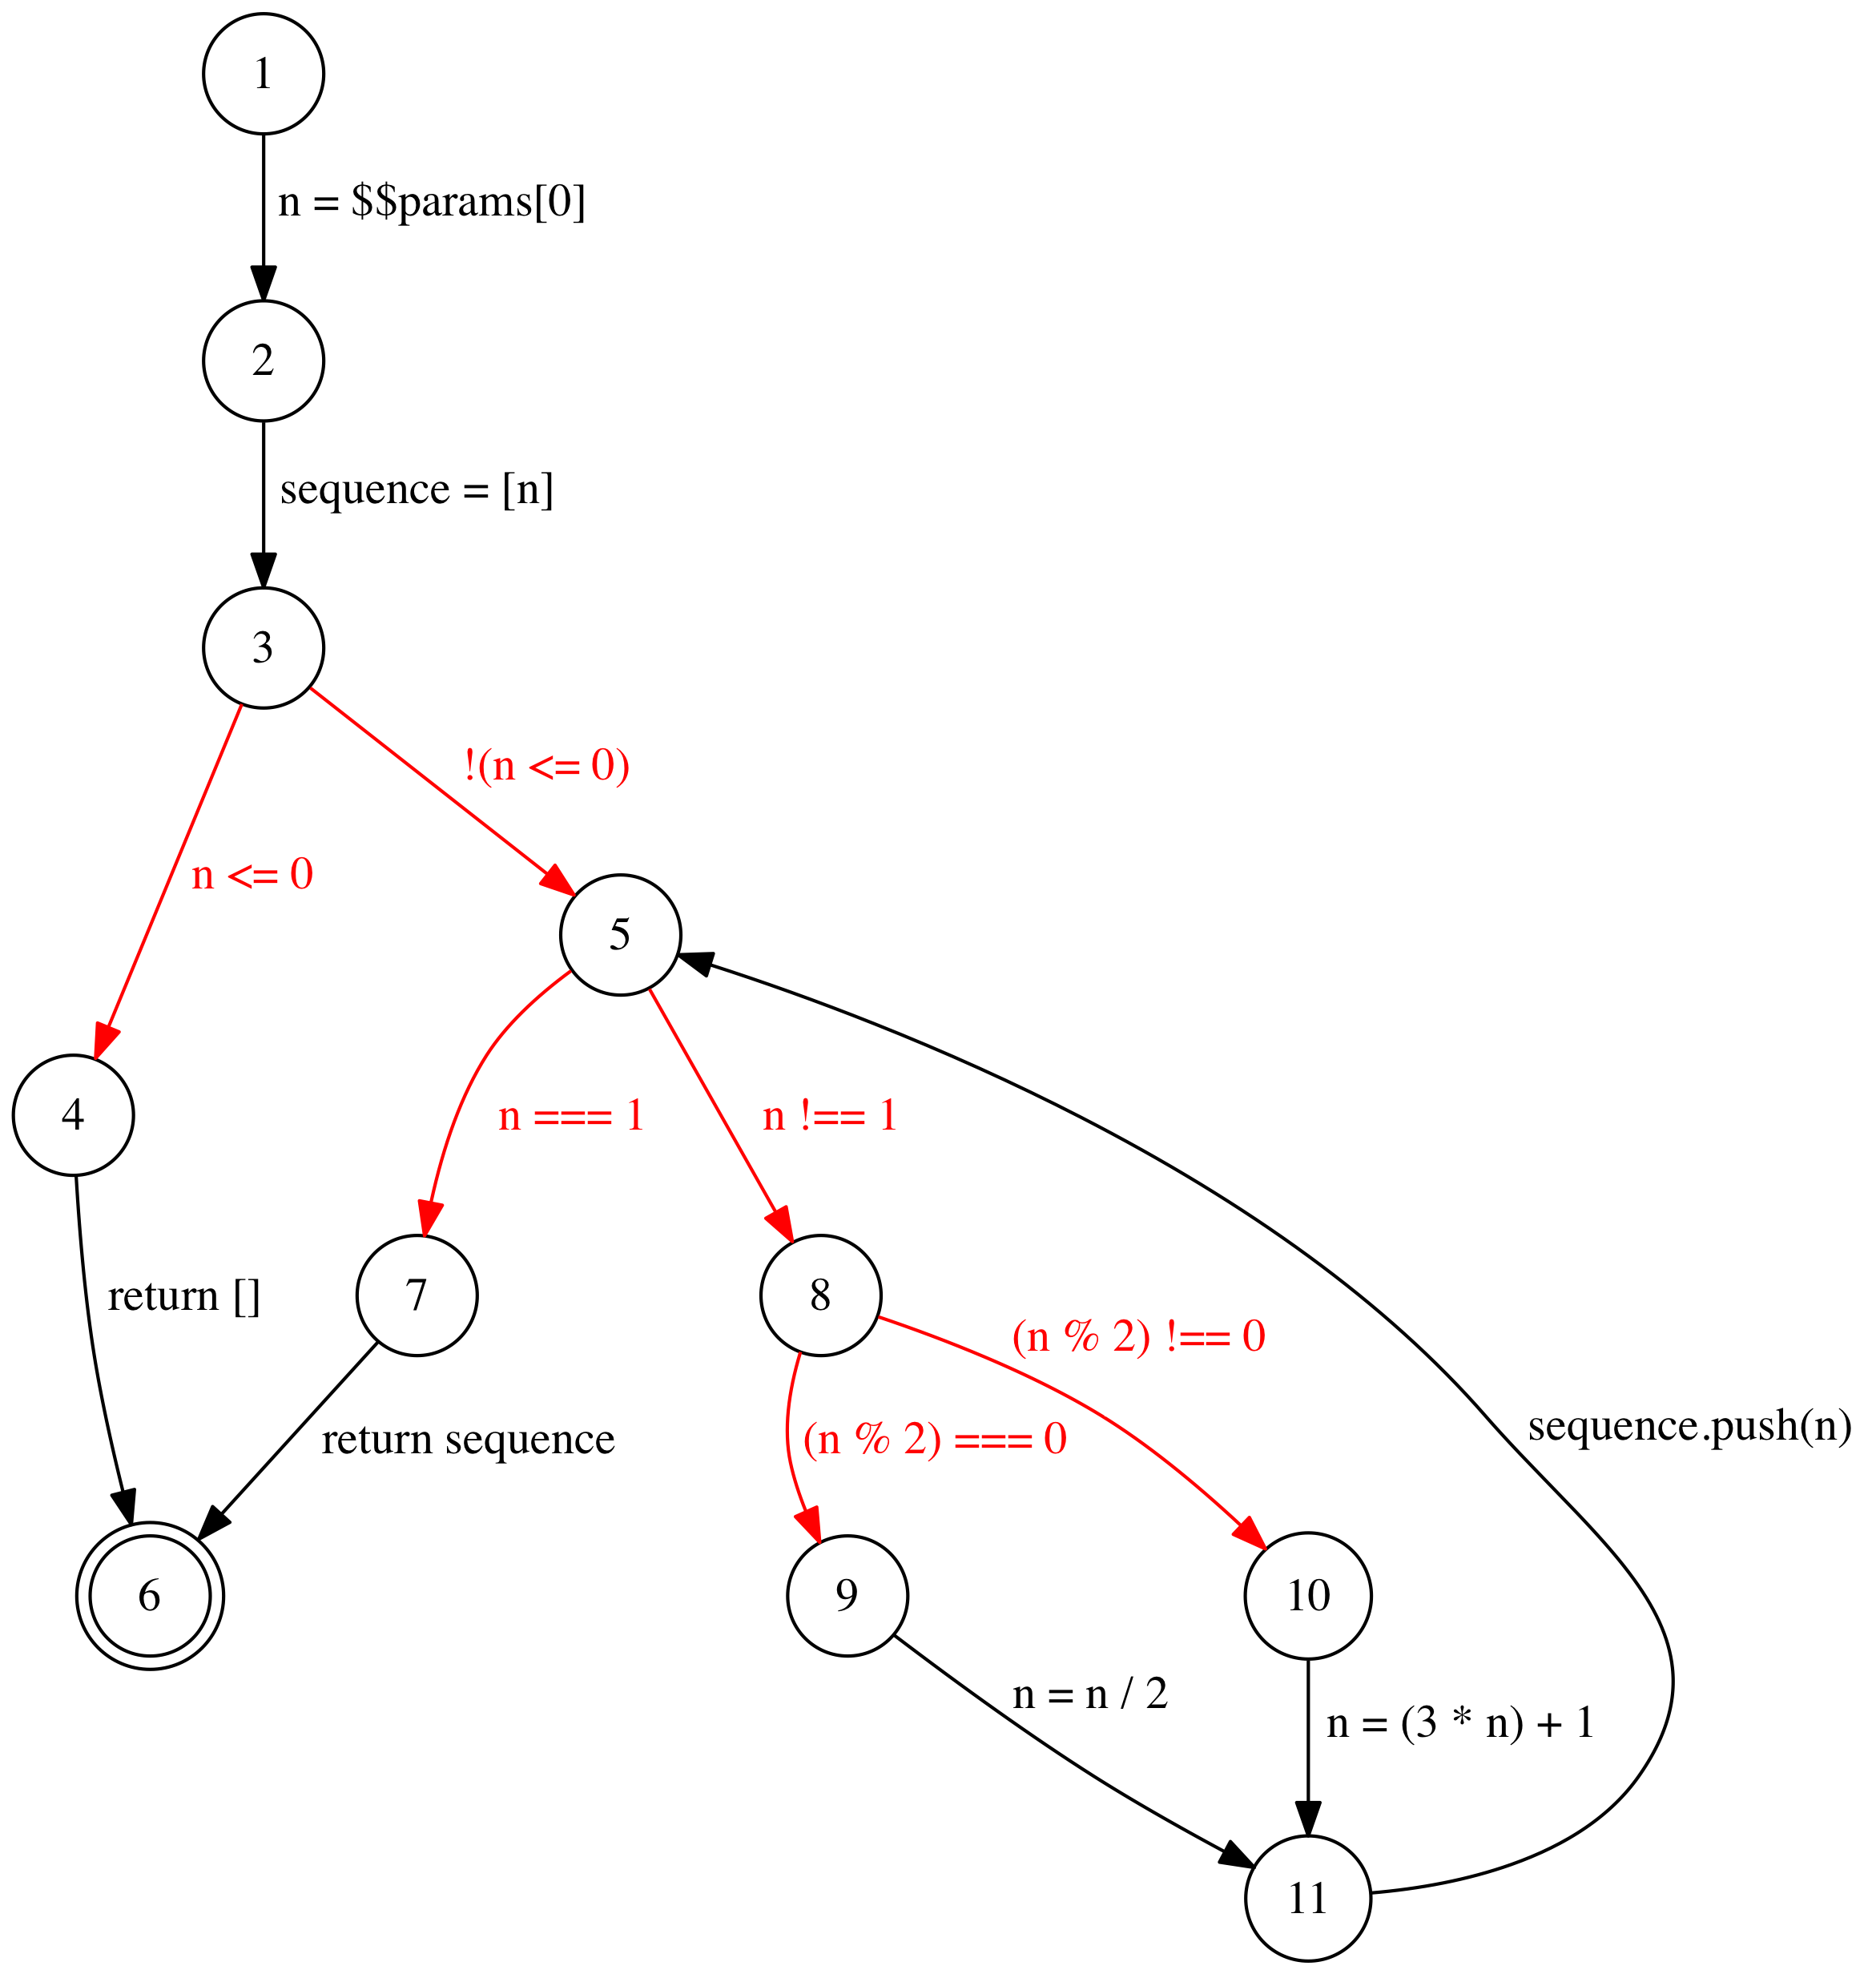
\includegraphics[width=\textwidth]{sections/appendix/images/collatz}
  \caption{The control flow graph of the \code{collatzSequence} function}
\end{figure}


\newpage
\subsubsection{JSON Export}

Exporting the control flow graph as JSON yields the following result:

\begin{minted}[baselinestretch=0.95,linenos,xleftmargin=0.6cm]{json}
{
  "program": {
    "flowGraph": {
      "nodes": [
        {
          "id": 1,
          "type": "Entry"
        },
        {
          "id": 2,
          "type": "SuccessExit"
        }
      ],
      "edges": [
        {
          "from": 1,
          "to": 2,
          "type": "Epsilon",
          "label": "",
          "data": null
        }
      ]
    }
  },
  "functions": [
    {
      "id": 1,
      "name": "collatzSequence",
      "flowGraph": {
        "nodes": [
          {
            "id": 4,
            "type": "Entry"
          },
          {
            "id": 5,
            "type": "SuccessExit"
          },
          {
            "id": 7,
            "type": "Normal"
          },
          {
            "id": 8,
            "type": "Normal"
          },
          {
            "id": 9,
            "type": "Normal"
          },
          {
            "id": 10,
            "type": "Normal"
          },
          {
            "id": 11,
            "type": "Normal"
          },
          {
            "id": 13,
            "type": "Normal"
          },
          {
            "id": 15,
            "type": "Normal"
          }
        ],
        "edges": [
          {
            "from": 4,
            "to": 7,
            "type": "Normal",
            "label": "n = $$params[0]",
            "data": {
              "type": "AssignmentExpression",
              "operator": "=",
              "left": {
                "type": "Identifier",
                "name": "n"
              },
              "right": {
                "type": "MemberExpression",
                "computed": true,
                "object": {
                  "type": "Identifier",
                  "name": "$$params"
                },
                "property": {
                  "type": "Literal",
                  "raw": "0",
                  "value": 0
                }
              }
            }
          },
          {
            "from": 7,
            "to": 8,
            "type": "Normal",
            "label": "sequence = [n]",
            "data": {
              "type": "VariableDeclarator",
              "id": {
                "type": "Identifier",
                "name": "sequence"
              },
              "init": {
                "type": "ArrayExpression",
                "elements": [
                  {
                    "type": "Identifier",
                    "name": "n"
                  }
                ]
              }
            }
          },
          {
            "from": 8,
            "to": 9,
            "type": "Conditional",
            "label": "n !== 1",
            "data": {
              "type": "BinaryExpression",
              "operator": "!==",
              "left": {
                "type": "Identifier",
                "name": "n"
              },
              "right": {
                "type": "Literal",
                "value": 1,
                "raw": "1"
              }
            }
          },
          {
            "from": 8,
            "to": 10,
            "type": "Conditional",
            "label": "n === 1",
            "data": {
              "type": "BinaryExpression",
              "operator": "===",
              "left": {
                "type": "Identifier",
                "name": "n"
              },
              "right": {
                "type": "Literal",
                "value": 1,
                "raw": "1"
              }
            }
          },
          {
            "from": 9,
            "to": 11,
            "type": "Conditional",
            "label": "(n % 2) === 0",
            "data": {
              "type": "BinaryExpression",
              "operator": "===",
              "left": {
                "type": "BinaryExpression",
                "operator": "%",
                "left": {
                  "type": "Identifier",
                  "name": "n"
                },
                "right": {
                  "type": "Literal",
                  "value": 2,
                  "raw": "2"
                }
              },
              "right": {
                "type": "Literal",
                "value": 0,
                "raw": "0"
              }
            }
          },
          {
            "from": 9,
            "to": 13,
            "type": "Conditional",
            "label": "(n % 2) !== 0",
            "data": {
              "type": "BinaryExpression",
              "operator": "!==",
              "left": {
                "type": "BinaryExpression",
                "operator": "%",
                "left": {
                  "type": "Identifier",
                  "name": "n"
                },
                "right": {
                  "type": "Literal",
                  "value": 2,
                  "raw": "2"
                }
              },
              "right": {
                "type": "Literal",
                "value": 0,
                "raw": "0"
              }
            }
          },
          {
            "from": 10,
            "to": 5,
            "type": "AbruptCompletion",
            "label": "return sequence",
            "data": {
              "type": "ReturnStatement",
              "argument": {
                "type": "Identifier",
                "name": "sequence"
              }
            }
          },
          {
            "from": 11,
            "to": 15,
            "type": "Normal",
            "label": "n = n / 2",
            "data": {
              "type": "AssignmentExpression",
              "operator": "=",
              "left": {
                "type": "Identifier",
                "name": "n"
              },
              "right": {
                "type": "BinaryExpression",
                "operator": "/",
                "left": {
                  "type": "Identifier",
                  "name": "n"
                },
                "right": {
                  "type": "Literal",
                  "value": 2,
                  "raw": "2"
                }
              }
            }
          },
          {
            "from": 13,
            "to": 15,
            "type": "Normal",
            "label": "n = (3 * n) + 1",
            "data": {
              "type": "AssignmentExpression",
              "operator": "=",
              "left": {
                "type": "Identifier",
                "name": "n"
              },
              "right": {
                "type": "BinaryExpression",
                "operator": "+",
                "left": {
                  "type": "BinaryExpression",
                  "operator": "*",
                  "left": {
                    "type": "Literal",
                    "value": 3,
                    "raw": "3"
                  },
                  "right": {
                    "type": "Identifier",
                    "name": "n"
                  }
                },
                "right": {
                  "type": "Literal",
                  "value": 1,
                  "raw": "1"
                }
              }
            }
          },
          {
            "from": 15,
            "to": 8,
            "type": "Normal",
            "label": "sequence.push(n)",
            "data": {
              "type": "CallExpression",
              "callee": {
                "type": "MemberExpression",
                "computed": false,
                "object": {
                  "type": "Identifier",
                  "name": "sequence"
                },
                "property": {
                  "type": "Identifier",
                  "name": "push"
                }
              },
              "arguments": [
                {
                  "type": "Identifier",
                  "name": "n"
                }
              ]
            }
          }
        ]
      }
    }
  ]
}
\end{minted}


\newpage
\subsubsection{Abstract Syntax Tree}

Shown below is the program's abstract syntax tree as generated by Esprima:

\begin{minted}[baselinestretch=0.975,linenos,xleftmargin=0.6cm]{json}
{
  "type": "Program",
  "body": [
    {
      "type": "FunctionDeclaration",
      "id": {
        "type": "Identifier",
        "name": "collatzSequence"
      },
      "params": [
        {
          "type": "Identifier",
          "name": "n"
        }
      ],
      "defaults": [],
      "body": {
        "type": "BlockStatement",
        "body": [
          {
            "type": "VariableDeclaration",
            "declarations": [
              {
                "type": "VariableDeclarator",
                "id": {
                  "type": "Identifier",
                  "name": "sequence"
                },
                "init": {
                  "type": "ArrayExpression",
                  "elements": [
                    {
                      "type": "Identifier",
                      "name": "n"
                    }
                  ]
                }
              }
            ],
            "kind": "var"
          },
          {
            "type": "IfStatement",
            "test": {
              "type": "BinaryExpression",
              "operator": "<=",
              "left": {
                "type": "Identifier",
                "name": "n"
              },
              "right": {
                "type": "Literal",
                "value": 0,
                "raw": "0"
              }
            },
            "consequent": {
              "type": "BlockStatement",
              "body": [
                {
                  "type": "ReturnStatement",
                  "argument": {
                    "type": "ArrayExpression",
                    "elements": []
                  }
                }
              ]
            },
            "alternate": null
          },
          {
            "type": "WhileStatement",
            "test": {
              "type": "BinaryExpression",
              "operator": "!==",
              "left": {
                "type": "Identifier",
                "name": "n"
              },
              "right": {
                "type": "Literal",
                "value": 1,
                "raw": "1"
              }
            },
            "body": {
              "type": "BlockStatement",
              "body": [
                {
                  "type": "IfStatement",
                  "test": {
                    "type": "BinaryExpression",
                    "operator": "===",
                    "left": {
                      "type": "BinaryExpression",
                      "operator": "%",
                      "left": {
                        "type": "Identifier",
                        "name": "n"
                      },
                      "right": {
                        "type": "Literal",
                        "value": 2,
                        "raw": "2"
                      }
                    },
                    "right": {
                      "type": "Literal",
                      "value": 0,
                      "raw": "0"
                    }
                  },
                  "consequent": {
                    "type": "BlockStatement",
                    "body": [
                      {
                        "type": "ExpressionStatement",
                        "expression": {
                          "type": "AssignmentExpression",
                          "operator": "=",
                          "left": {
                            "type": "Identifier",
                            "name": "n"
                          },
                          "right": {
                            "type": "BinaryExpression",
                            "operator": "/",
                            "left": {
                              "type": "Identifier",
                              "name": "n"
                            },
                            "right": {
                              "type": "Literal",
                              "value": 2,
                              "raw": "2"
                            }
                          }
                        }
                      }
                    ]
                  },
                  "alternate": {
                    "type": "BlockStatement",
                    "body": [
                      {
                        "type": "ExpressionStatement",
                        "expression": {
                          "type": "AssignmentExpression",
                          "operator": "=",
                          "left": {
                            "type": "Identifier",
                            "name": "n"
                          },
                          "right": {
                            "type": "BinaryExpression",
                            "operator": "+",
                            "left": {
                              "type": "BinaryExpression",
                              "operator": "*",
                              "left": {
                                "type": "Literal",
                                "value": 3,
                                "raw": "3"
                              },
                              "right": {
                                "type": "Identifier",
                                "name": "n"
                              }
                            },
                            "right": {
                              "type": "Literal",
                              "value": 1,
                              "raw": "1"
                            }
                          }
                        }
                      }
                    ]
                  }
                },
                {
                  "type": "ExpressionStatement",
                  "expression": {
                    "type": "CallExpression",
                    "callee": {
                      "type": "MemberExpression",
                      "computed": false,
                      "object": {
                        "type": "Identifier",
                        "name": "sequence"
                      },
                      "property": {
                        "type": "Identifier",
                        "name": "push"
                      }
                    },
                    "arguments": [
                      {
                        "type": "Identifier",
                        "name": "n"
                      }
                    ]
                  }
                }
              ]
            }
          },
          {
            "type": "ReturnStatement",
            "argument": {
              "type": "Identifier",
              "name": "sequence"
            }
          }
        ]
      },
      "rest": null,
      "generator": false,
      "expression": false
    }
  ]
}
\end{minted}



\end{document}
